\documentclass{book}
\usepackage[english]{babel}
\usepackage{amsmath,amssymb,graphicx,enumerate,bbm,latexsym,theorem}

%%%%%%%%%% Start TeXmacs macros
\newcommand{\Tau}{\mathrm{T}}
\newcommand{\assign}{:=}
\newcommand{\mathd}{\mathrm{d}}
\newcommand{\mathe}{\mathrm{e}}
\newcommand{\mathi}{\mathrm{i}}
\newcommand{\mathpi}{\pi}
\newcommand{\nobracket}{}
\newcommand{\nospace}{}
\newcommand{\tmaffiliation}[1]{\\ #1}
\newcommand{\tmname}[1]{\textsc{#1}}
\newcommand{\tmop}[1]{\ensuremath{\operatorname{#1}}}
\newcommand{\tmsamp}[1]{\textsf{#1}}
\newcommand{\tmtextit}[1]{{\itshape{#1}}}
\newcommand{\tmverbatim}[1]{{\ttfamily{#1}}}
\newenvironment{enumeratenumeric}{\begin{enumerate}[1.] }{\end{enumerate}}
\newenvironment{enumerateroman}{\begin{enumerate}[i.] }{\end{enumerate}}
\newenvironment{proof}{\noindent\textbf{Proof\ }}{\hspace*{\fill}$\Box$\medskip}
\newtheorem{corollary}{Corollary}
\newtheorem{definition}{Definition}
{\theorembodyfont{\rmfamily}\newtheorem{example}{Example}}
\newtheorem{lemma}{Lemma}
\newtheorem{proposition}{Proposition}
\newtheorem{theorem}{Theorem}
%%%%%%%%%% End TeXmacs macros

%


\begin{document}

\title{Wavelet Analysis and Its Application in CFD}

\author{
  LIU Zeyu
  \tmaffiliation{College of Engineering, Peking University{\tmsamp{}}}
}

\maketitle

\chapter*{Prologue}

The concept of wavelet is originated from Fourier analysis. The classical
Fourier transform
\[ \hat{f} (\gamma) = \int_{- \infty}^{+ \infty} f (x) \mathe^{- 2 \mathpi
   \mathi \gamma x} \mathd x \]
converts information to the \tmtextit{frequency space}. However, the Fourier
transform is not localized in both physical space and frequency space. One
method of obtain local information on physical space of a signal is the
Fourier transform with a window function $g (t - b)$:
\[ (G_{a, b} f) (\gamma) \assign \int_{- \infty}^{+ \infty} f (t) e^{- 2
   \mathpi \mathi \gamma x} g_a (t - b) \mathd t \]
where
\[ g_a (t - b) \assign \frac{1}{2 \sqrt{\mathpi a}} \mathe^{- \frac{x^2}{4 a}}
   . \]
The above transform is also called \tmtextit{Gabor transform}. The shortcoming
of Gabor transform is that it has only fixed window, so it is not suitable for
signals with singularity or severe oscillation. Inspired by the above methods,
wavelet transform provides a systematical tool of analyzing unstable signals.

\part{Mathematical Foundations of Wavelet Analysis}

\chapter{Basic{} Concepts of Wavelet}

\section{An Abstract Way of Introducing Discrete Wavelet Transform}

\subsection{Wavelet}

In general, the Hilbert space has the property described in the following
theorem:{\cite{christensen2010functions}}

\begin{theorem}[Existence of orthonormal bases]
  Every separable Hilbert space
  {\tmname{{\tmsamp{\tmverbatim{}}}}}$\mathcal{H}$ has an orthonormal basis.
\end{theorem}

Discrete wavelet transform provides a way of constructing orthonormal bases in
$L^2 (\mathbbm{R})$ with a special structure: all of them are scaled and
translated version of a fixed function. The character that distinguishes bases
with wavelet structure from other orthonormal bases in $L^2 (\mathbbm{R})$ is
that the relevant function can be approximated well by finite partial sums,
and even with just a few nonzero coefficients.

\begin{definition}[Wavelet]
  Let $\psi \in L^2 (\mathbbm{R})$.
  \begin{enumerateroman}
    \item For $j, k \in \mathbbm{Z}$, define the function $\psi_{j, k}$ by
    \[ \psi_{j, k} \assign 2^{j / 2} \psi (2^j x - k) \quad x \in \mathbbm{R}.
    \]
    \item The function $\psi$ is called a wavelet if the functions $\{
    \psi_{j, k} \}_{j, k \in \mathbbm{Z}}$ form an orthonormal basis for $L^2
    (\mathbbm{R})$.
  \end{enumerateroman}
\end{definition}

In terms of the translation operator $T_k$ and the dilation operator $D$, we
have
\[ \psi_{j, k} = D^j T_k \psi \quad j, k \in \mathbbm{Z}. \]


The systematical theory of constructing wavelet began in middle 1980s, but the
first wavelet is constructed much earlier and it is proved by Haar in 1910
that the following function consistutes an example of wavelet.

\begin{example}[Haar Function]
  The \tmtextit{Haar function} is defined by \[ \psi (x) = \left\{
     \begin{array}{cc}
       1 & \text{if} \quad 0 \leqslant x < 1 / 2\\
       - 1 & \text{if} \quad 1 / 2 \leqslant x < 1\\
       0 & \text{otherwise.}
     \end{array} \right. \]
\end{example}

It is very complicated to verify that Haar function is wavelet, and it is
mentioned here just to point out the existence of wavelet, and an illustration
on how Haar function forms a wavelet is in Section \ref{sec:haarWavelet}.

\subsection{Multiresolution Analysis}

Multiresolution analysis is a general tool to construct wavelet orthonormal
bases. A multiresolution analysis consists of a collection of conditions on
certain subspaces of $L^2 (\mathbbm{R})$, and an associated function $\phi \in
L^2 (\mathbbm{R})$.

\begin{definition}[Multiresolution Analysis]
  \label{def:multiresolutionAnalysis}A multiresolution analysis for $L^2
  (\mathbbm{R})$ consists of a squence of closed subspaces $\{ V_i \}_{i \in
  \mathbbm{Z}}$ of $L^2 (\mathbbm{R})$ and a function $\phi \in V_0$, such
  that the following conditions hold:
  \begin{enumerateroman}
    \item The space $V_j$ are nested, i.e.,
    \[ \cdots \subset V_{- 1} \subset V_0 \subset V_1 \subset \cdots . \]
    \item $\overline{\bigcup_{j \in \mathbbm{Z}} V_j} = L^2 (\mathbbm{R})$ and
    $\bigcap_{j \in \mathbbm{Z}} V_j = \{ 0 \} .$
    
    \item $\forall j \in \mathbbm{Z}$, $V_{j + 1} = D (V_j)$.
    
    \item $\forall k \in \mathbbm{Z}$, $f \in V_0 \Rightarrow T_k f \in V_0$.
    
    \item $\{ T_k \phi \}_{k \in \mathbbm{Z}}$ is an orthonormal basis for
    $V_{0.}$
  \end{enumerateroman}
\end{definition}

A closer look at the condition the condition in Definition
\ref{def:multiresolutionAnalysis} reveals that the choice of the function
$\phi$ in a multiresolution analysis acturally determines the space $V_j$
uniquely:

\begin{lemma}[The Space $V_j$]
  \label{lem:spaceVj}Assume that the conditions (iii) and (iv) in Definition
  \ref{def:multiresolutionAnalysis} are satisfied. Then the following hold:
  \begin{enumerateroman}
    \item $V_j = D^j (V_0)$ for all $j \in \mathbbm{Z}$.
    
    \item $V_j = \overline{\tmop{span} \{ D^j T_k \phi \}_{k \in
    \mathbbm{Z}}}$ for all $j \in \mathbbm{Z}.$
  \end{enumerateroman}
\end{lemma}

\begin{proof}
  For $j \in \mathbbm{N}$:
  \[ V_j = D (V_{j - 1}) = D D (V_{j - 2}) = \cdots = D^j (V_0), \]
  and for $j < 0$, (i) holds similarly.
  \begin{equation}
    V_j = D^j (V_0) = D^j (\overline{\tmop{span} \{ T_k \phi \}_{k \in
    \mathbbm{Z}}}) = \overline{\tmop{span} \{ D^j T_k \phi \}_{k \in
    \mathbbm{Z}}} . \label{Vj}
  \end{equation}
  
\end{proof}

Lemma \ref{lem:spaceVj}(ii) shows that the space $V_j$ in a multiresolution
analysis are uniquely determined by the function $\phi$, so we say that the
function $\phi$ \tmtextit{generates the multiresolution analysis}. Later in
this Chapter, it will shown that only very special function $\phi$ can
generate multiresolution analysis.

\begin{example}[Haar Multiresolution Analysis]
  \label{eg:haarMRA}We can define a multiresolution analysis by
  \[ \left\{ \begin{array}{lll}
       \phi & \assign & \chi_{[0, 1)} ;\\
       V_j & \assign & \{ f \in L^2 (\mathbbm{R}) f \tmop{is} \tmop{constant}
       \tmop{on} [2^{- j} k, 2^{- j} (k + 1)), \forall k \in \mathbbm{Z} \} .
     \end{array} \right. \]
  Note that the Haar wavelet can be written as
  \begin{eqnarray*}
    \psi (x) & = & \chi_{[0, 1 / 2)} (x) - \chi_{[1 / 2, 1)} (x)\\
    & = & \chi_{[0, 1)} (2 x) - \chi_{[0, 1)} (2 x - 1)\\
    & = & \frac{1}{\sqrt{2}} (D \chi_{[0, 1)} (x) - D T_1 \chi_{[0, 1)}
    (x))\\
    & = & \frac{1}{\sqrt{2}} (D \phi (x) - D T_1 \phi (x))
  \end{eqnarray*}
\end{example}

In order to construct an orthonormal basis for $L^2 (\mathbbm{R})$ with
multiresolution analysis, we need to consider a class of vector space $W_j$
associated with \{$V_j \}_{j \in \mathbbm{Z}} \nobracket$:

\begin{definition}[The Space $W_j$]
  Assume that $V_j$ is a sequence of closed subspace of $L^2 (\mathbbm{R})$
  and that the condition (i) in Definition \ref{def:multiresolutionAnalysis}
  is satisfied. For any $j \in \mathbbm{Z}$, let $W_j$ denote the orthogonal
  complement of $V_j$ with respect to $V_{j + 1}$, i.e.,
  \[ W_j \assign \{ f \in V_{j + 1} | \langle f, g \rangle = 0, \forall g \in
     V_j \} . \]
  We denote the orthogonal projection of $L^2 (\mathbbm{R})$ onto $W_j$ by
  $Q_j$.
\end{definition}

The above construction of space $W_j$ is very similar to Gram-Schmidt process
in finite-dimensional linear algebra. However, in infinite-dimensional vector
spaces, the Gram-Schmidt process does not make sense in general. The
multiresolution analysis provides a special condition with which a process
similar to Gram-Schmidt process is feasible.

It turns out that the space $W_0$ plays a very special role in wavelet
analysis. In fact, the next result shows that in order to obtain an
orthonormal basis $\{ D^j T_k \psi \}_{j, k \in \mathbbm{Z}}$ for $L^2
(\mathbbm{R})$, it is enough to find a function $\psi \in W_0$ such that $\{
\psi (\cdot - k) \}_{k \in \mathbbm{Z}}$ is an orthonormal basis for $W_{0.}$

\begin{proposition}
  Assume that the function $\phi \in L^2 (\mathbbm{R})$ generates a
  multiresolution analysis. Let $\psi \in L^2 (\mathbbm{R})$ and suppose that
  $\{ T_k \psi \}_{k \in \mathbbm{Z}}$ form an orthonormal basis for $W_0$.
  Then the following holds:
  \begin{enumerateroman}
    \item For each $j \in \mathbbm{Z}$, the functions $\{ D^j T_k \psi \}_{k
    \in \mathbbm{Z}}$ form an orthonormal basis for $W_j$.
    
    \item The functions $\{ D^j T_k \psi \}_{j, k \in \mathbbm{Z}}$ form an
    orthonormal basis for $L^2 (\mathbbm{R})$, i.e., $\psi$ is a wavelet.
    
    \item The functions $\{ T_k \phi \}_{k \in \mathbbm{Z}} \cup \{ D^j T_k
    \psi \}_{j \in \mathbbm{N}, k \in \mathbbm{Z}}$ form an orthonormal basis
    for $L^2 (\mathbbm{R})$.{\hspace*{\fill}}
  \end{enumerateroman}
\end{proposition}

Since function $\psi$ is a wavelet and function $\phi$ generates the
corresponding multiresolution analysis, it is important to point out the
relationship between the two functions. The following in this section also
shows the general method of constructing a multiresolution analysis.

\begin{proposition}[Scaling Function]
  Assume that the function $\phi \in L^2 (\mathbbm{R})$ generates a
  multiresolution analysis. Then there exists a 1-periodic function $H_0 \in
  L^2 (0, 1)$ such that
  \begin{equation}
    \hat{\phi} (2 \gamma) = H_0 (\gamma) \hat{\phi} (\gamma)
    \label{scalingEquation}
  \end{equation}
\end{proposition}

Solution to Equation (\ref{scalingEquation}) is called a \tmtextit{scaling
function}, or said to be \tmtextit{refinable}. Formulated in this language, a
necessary condition for a function $\phi$ to generate a multiresolution
analysis is that $\phi$ is a scaling function. Later it will be shown that
that condition added up with two extra conditions can become sufficient. The
following theorem provides a concrete statement on how to generate a wavelet
with Equation (\ref{scalingEquation}).

\begin{theorem}[Wavelet Orthonormal Basis]
  \label{thm:constructionWavelet}Assume that $\phi \in L^2 (\mathbbm{R})$
  generates a multiresolution analysis, and let $H_0 \in L^2 (0, 1)$ be a
  1-periodic function satisfying the scaling equation (\ref{scalingEquation}).
  Define the 1-periodic function $H_1$ by
  \begin{equation}
    H_1 \assign \overline{H_0 \left( \gamma + \frac{1}{2} \right)} \mathe^{- 2
    \mathpi \mathi \gamma} \label{h1}
  \end{equation}
  Also define the function $\psi$ via
  \begin{equation}
    \hat{\psi} (2 \gamma) \assign H_1 (\gamma) \hat{\phi} (\gamma) .
    \label{psiScaling}
  \end{equation}
  Then the following holds:
  \begin{enumerateroman}
    \item $\{ T_k \psi \}_{k \in \mathbbm{Z}}$ is an orthonormal basis for
    $W_0$.
    
    \item $\{ D^j T_k \psi \}_{j, k \in \mathbbm{Z}}$ is orthonormal basis for
    $L^2 (\mathbbm{R})$, i.e., $\psi$ is a wavelet.
  \end{enumerateroman}
\end{theorem}

The direct way of defining the wavelet $\psi$ is applying inverse Fourier
transform on $\hat{\psi} (\gamma)$:

\begin{theorem}[Explicit Expression for the Wavelet]
  Assume that (\ref{psiScaling}) holds for a 1-periodic function $H_1 \in L^2
  (0, 1)$,
  \[ H_1 (\gamma) = \sum_{k \in \mathbbm{Z}} d_k \mathe^{2 \mathpi \mathi k
     \gamma} . \]
  Then
  \begin{equation}
    \psi (x) = \sqrt{2} \sum_{k \in \mathbbm{Z}} d_k D T_{- k} \phi (x) = 2
    \sum_{k \in \mathbbm{Z}} d_k \phi (2 x + k) \quad x \in \mathbbm{R}.
    \label{psiScalingExplicit}
  \end{equation}
\end{theorem}

The Equation (\ref{psiScalingExplicit}) provides the method of finding the
wavelet $\psi$ whenever the function $H_0$ has been calculated. In most cases
of practical interest, $H_0$ is actually a trigonometric polynomial:
\[ H_0 (\gamma) = \sum_{k = - N}^N c_k \mathe^{2 \mathpi \mathi k \gamma} . \]
The explicit expression of the wavelet in (\ref{psiScalingExplicit})
immediately leads to a criterion for how to obtain a compactly supported
wavelet:

\begin{corollary}[Compactly Supported Wavelet]
  Assume that the function $\phi \in L^2 (\mathbbm{R})$ is compactly supported
  and generates a multiresolution analysis. Assume further that the function
  $H_0$ in the scaling equation (\ref{scalingEquation}) is a trigonometric
  polynomial. Then the wavelet $\psi$ in (\ref{psiScalingExplicit}) is
  compactly supported.
\end{corollary}

\begin{example}[Haar Wavelet]
  The previous conclusions can all be applied to the case of Haar wavelet.
\end{example}

Since a multiresolution analysis is uniquely characterized by the scaling
function $\phi$, it is natural to examine how to formulate the multiresolution
analysis conditions directly in terms of conditions on the function $\phi$.
Such conditions are:

\begin{theorem}[Construction of Multiresolution Analysis]
  \label{thm:constructionMRA}Let $\phi \in L^2 (\mathbbm{R})$. Define the
  spaces $V_j$ by (\ref{Vj}), and assume that the following conditions holds:
  \begin{enumerateroman}
    \item $\inf_{\gamma \in (- \varepsilon, \varepsilon)} | \hat{\phi}
    (\gamma) | > 0$ for some $\varepsilon > 0$;
    
    \item the scaling equation
    \[ \hat{\phi} (2 \gamma) = H_0 (\gamma) \hat{\phi} (\gamma) \]
    is satisfied with a bounded 1-periodic function $H_0$;
    
    \item $\{ T_k \phi \}_{k \in \mathbbm{Z}}$ form an orthonormal system.
  \end{enumerateroman}
\end{theorem}

\begin{theorem}[Characterization of Orthonormal System $\{ T_k \phi \}_{k \in
\mathbbm{Z}}$]
  Let $\phi \in L^2 (\mathbbm{R})$. Then $\{ T_k \phi \}_{k \in \mathbbm{Z}}$
  is an orthornormal system if and only if
  \[ \sum_{k \in \mathbbm{Z}} | \hat{\phi} (\gamma + k) |^2 = 1 \quad \gamma
     \in \mathbbm{R} \]
\end{theorem}

\subsection{Vanishing Moments and Daubechies' Wavelet}

This section mainly discusses the properties that make wavelet analysis useful
in signal processing, and the construction by Ingrid Daubechies.

Since the functions $\{ T_k \phi \}_{k \in \mathbbm{Z}} \cup \{ D^j T_k \psi
\}_{j \in \mathbbm{N}, k \in \mathbbm{Z}}$ form an orthonormal basis for $L^2
(\mathbbm{R})$, we know that any $f \in L^2 (\mathbbm{R})$ has the
representation
\begin{equation}
  f = \sum_{k \in \mathbbm{Z}} \langle f, T_k \phi \rangle T_k \phi + \sum_{j
  = 1}^{\infty} \sum_{k \in \mathbbm{Z}} \langle f, \psi_{j, k} \rangle
  \psi_{j, k} . \label{representation}
\end{equation}
All information about the function $f$ is stored in the coefficients
\[ \{ \langle f, T_k \phi \rangle \}_{k \in \mathbbm{Z}}^{} \cup \{ \langle f,
   \psi_{j, k} \rangle \}_{j \in \mathbbm{N}, k \in \mathbbm{Z}} . \]
However, in practice computers can only process finite sequence, so one has to
select a finite number of coefficients to keep. In most situation of practical
interest, such as the wavelet generated by a compactly supported scaling
function $\phi \in L^2 (\mathbbm{R})$, the sequence $\{ \langle f, T_k \phi
\rangle \}_{k \in \mathbbm{Z}}$ is actually finite, thus the problems is how
to deal with the infinite sequence $\{ \langle f, \psi_{j, k} \rangle \}_{j
\in \mathbbm{N}, k \in \mathbbm{Z}}$. This is usually done by
\tmtextit{thresholding}{\cite{schneider2010wavelet}}: we choose a certain
$\varepsilon > 0$ and keep only the coefficients in (\ref{representation})
under condition:
\begin{equation}
  | \langle f, \psi_{j, k} \rangle | \geqslant \varepsilon .
  \label{thresholdingCondition}
\end{equation}
By convergence of (\ref{representation}) the coefficients $\{ \langle f,
\psi_{j, k} \rangle \}_{j, k \in \mathbbm{Z}} \subset \ell^2$, so only finite
number of indices $(j, k) \in \mathbbm{Z} \times \mathbbm{Z}$ satisfy
(\ref{thresholdingCondition}). A key feature of wavelet theory is that it is
often posible to choose the wavelet $\psi$ such that many of the coefficients
$\{ \langle f, \psi_{j, k} \rangle \}_{j \in \mathbbm{N}, k \in \mathbbm{Z}}$
are small.

\begin{example}[Haar Wavelet]
  For Haar wavelet, we have (\ref{representation}) as
  \[ \langle f, \psi_{j, k} \rangle \psi_{j, k} (x) = 2^{j / 2} \langle f,
     \psi_{j, k} \rangle \psi (2^j x - k), \]
  and it can be shown that
  \begin{eqnarray*}
    d_{j, k} & \assign & 2^{j / 2} \langle f, \psi_{j, k} \rangle\\
    & = & \frac{1}{2} (\tmop{average} \tmop{of} f \tmop{over} [2^{- j} k,
    2^{- j} (k + 1 / 2)) - \tmop{average} \tmop{of} f \tmop{over} [2^{- j} (k
    + 1 / 2), 2^{- j} (\nobracket k + 1)) .
  \end{eqnarray*}
  Since
  \[ \langle f, \psi_{j, k} \rangle = 2^{- j / 2} d_{j, k} \quad j \geqslant 1
     \quad k \in \mathbbm{Z}, \]
  most coefficients in (\ref{representation}) are very small if $f$ is
  continuous or oscillates slightly.
\end{example}

In order to find wavelets that are better than Haar wavelet, we need to
introduce \tmtextit{vanishing moment} first.

\begin{definition}[Vanishing Moment]
  Let $N \in \mathbbm{N}$. A function $\psi$ has $N$ vanishing moments if
  \[ \int_{- \infty}^{+ \infty} x^{\ell} \psi (x) \mathd x = 0 \quad
     \tmop{for} \ell = 0, 1, \ldots, N - 1. \]
\end{definition}

The Haar wavelet has only one vanishing moment. We have the following result
showing that only relatively few coefficients $\langle f, \psi_{j, k} \rangle$
will be large if $\psi$ has a large number of vanishing moments.

\begin{theorem}[Decay of Wavelet Coefficients]
  \label{thm:decay}Assume that the function $\psi \in L^2 (\mathbbm{R}) $ is
  compactly supported and has $N$ vanishing moments. Then, for any $N$times
  differentiable function $f \in L^2 (\mathbbm{R})$ for which the $N$th
  derivative $f^{(N)}$ is bounded, there exists a constant $C > 0$ such that
  \begin{equation}
    | \langle f, \psi_{j, k} \rangle | \leqslant C 2^{- j N} 2^{- j / 2} \quad
    \forall j \geqslant 1 \quad k \in \mathbbm{Z} \label{basicEstimate}
  \end{equation}
\end{theorem}

The proof of Theorem (\ref{thm:decay}) is complicated
{\cite{walnut2013introduction}}, but the result shows clearly that: the higher
number of vanishing moments a wavelet has, the fewer coefficients $\{ \langle
f, \psi_{j, k} \rangle \}_{j \in \mathbbm{N}, k \in \mathbbm{Z}}$ remain after
thresholding. Another import theorem is provided by
{\cite{walnut2013introduction}}:

\begin{theorem}[Vanishing Moment]
  \label{thm:vanishingMoment}Let $\phi$ be a compactly supported scaling
  function associated with a multiresolution analysis, and let $\psi$ be the
  associated wavelet as in (\ref{scalingEquation}). Then the following are
  equivalent:
  \begin{enumerateroman}
    \item $\psi$ has $N$ vanishing moments.
    
    \item The function $H_0$ can be factorized
    \begin{equation}
      H_0 (\gamma) = \left( \frac{1 + \mathe^{- 2 \mathpi \mathi \gamma}}{2}
      \right)^N L (\gamma) \label{vanishingMomentH}
    \end{equation}
    for some 1-periodic trigonometric polynomial $L$.
  \end{enumerateroman}
\end{theorem}

Combining Theorem (\ref{thm:constructionMRA}) and Theorem
(\ref{thm:vanishingMoment}) produces one approach to construct a wavelet
$\psi$ having $N$ vanishing moments by searching for a proper 1-periodic
function $H_0 \in L^2 (0, 1)$. Then
\[ \hat{\phi} (\gamma) = H_0 (\gamma / 2) \hat{\phi} (\gamma / 2) = H_0
   (\gamma / 2) H_0 (\gamma / 4) \hat{\phi} (\gamma / 4) = H_0 (\gamma / 2)
   H_0 (\gamma / 4) H_0 (\gamma / 8) \hat{\phi} (\gamma / 8), \]
and finally for any $K \in \mathbbm{N}$
\[ \hat{\phi} (\gamma) = H_0 (\gamma / 2) H_0 (\gamma / 4) H_0 (\gamma / 8)
   \cdots H_0 (\gamma / 2^K) \hat{\phi} (\gamma / 2^K) = \hat{\phi} (\gamma /
   2^K) \prod_{j = 1}^K H_0 (\gamma / 2^j) . \]
It can be proved that the following limit process is feasible
\begin{eqnarray*}
  \hat{\phi} (\gamma) & = & \lim_{K \rightarrow \infty} \left( \hat{\phi}
  (\gamma / 2^K) \prod_{j = 1}^K H_0 (\gamma / 2^j) \right)\\
  & = & \hat{\phi} (0) \prod_{j = 1}^{\infty} H_0 (\gamma / 2^j) .
\end{eqnarray*}
This also ensures the uniqueness (up to a scalar multiplication) of scaling
function $\phi$ since once $\hat{\phi} (0)$ is given, all other values are
determined.

The \tmtextit{Daubechies' wavelets} are the best known constructions based on
the above idea. First denote $P_{N - 1}, N \in \mathbbm{N}$ by
\[ P_{N - 1} (y) = \sum_{k = 0}^{N - 1} \frac{(2 N - 1) !}{k! (2 N - 1 - k) !}
   y^k (1 - y)^{N - 1 - k}, \]
then {\cite{daubechies1992ten}} provides another important theorem:

\begin{theorem}[Daubechies' Wavelets]
  For any $N \in \mathbbm{N}$, there exists a trigonometric polynomial $L$
  such that
  \begin{equation}
    | L (\gamma) |^2 = P_{N - 1} (\sin^2 \mathpi \gamma) . \label{daubechiesL}
  \end{equation}
  With such a choice for $L$, the following hold:
  \begin{enumerateroman}
    \item The function $H_0$ given by (\ref{vanishingMomentH}) is associated
    with a multiresolution analysis.
    
    \item With $H_0$ as in (i), the wavelet $\psi$ given in Theorem
    \ref{thm:constructionWavelet} has $N$ vanishing moments, and support in
    $[0, 2 N - 1] .$
  \end{enumerateroman}
\end{theorem}

\begin{example}[The Polynomial $P_{N - 1}$]
  It can be calculated that:
  \begin{eqnarray*}
    P_0 (y) & = & 1\\
    P_1 (y) & = & 1 + 2 y\\
    P_2 (y) & = & 1 + 3 y + 6 y^2
  \end{eqnarray*}
\end{example}

Daubechies further provides a procedure called \tmtextit{spectral
factorization} to find the trigonometric polynomial $L$ satisfying
(\ref{daubechiesL}).

\begin{example}[Spectral Factorization with $N = 1$]
  For $N = 1$, $| L (\gamma) |^2 = 1$, which is satisfied for $L (\gamma) = -
  1$. Via (\ref{vanishingMomentH}), this leads to
  \[ H_0 (\gamma) = \frac{1 + \mathe^{- 2 \mathpi \mathi \gamma}}{2} L
     (\gamma) = \frac{- 1 - \mathe^{- 2 \mathpi \mathi \gamma}}{2} . \]
  We can calculate $H_1$:
  \begin{eqnarray*}
    H_1 (\gamma) & = & \overline{H_0 \left( \gamma + \frac{1}{2} \right)}
    \mathe^{- 2 \mathpi \mathi \gamma}\\
    & = & \overline{\frac{- 1 - \mathe^{- 2 \mathpi \mathi (\gamma + 1 /
    2)}}{2}} \mathe^{- 2 \mathpi \mathi \gamma}\\
    & = & \frac{1 - \mathe^{- 2 \mathpi \mathi \gamma}}{2}\\
    & = & \sum_{k = - 1}^0 d_k \mathe^{2 \mathpi \mathi k x},
  \end{eqnarray*}
  where $d_0 = 1 / 2, d_{- 1} = - 1 / 2$. By (\ref{psiScalingExplicit}), the
  associated wavelet is
  \[ \psi (x) = \sqrt{2} \sum_{k = - 1}^0 d_k D T_{- k} \phi (x) = \phi (2 x)
     - \phi (2 x - 1), \]
  which is exactly the expression for the Haar wavelet in Example
  \ref{eg:haarMRA}.
\end{example}

\section{An Elementary Way of Introducing Wavelet Theory}

This section is mainly according to
{\cite{WangJizeng2001,williams1994introduction}}, and provides another way of
defining (orthogonal) wavelet which is better for programming, but lacks
mathematical rigorousness.

\subsection{Example: Haar Wavelet}

\label{haarWavelet}This section is an demonstration on how to approximate an
arbitrary function $f$ in $L^2 (\mathbbm{R})$ by linear combination of Haar
wavelet {\cite{daubechies1992ten}}. First, any function $f \in L^2
(\mathbbm{R})$ can be arbitrarily well approximated by a function with compact
support which is piecewise constant on the interval $[\ell 2^{- j}, (\ell + 1)
2^{- j})$ (it suffices to take the support and $j$ large enough). As a result,
we consider the following piecewise constant function: assume $f$ to be
supported on $[- 2^{J_1}, 2^{J_1}]$, and to be piecewise constant on $[\ell
2^{- J_0}, (\ell + 1) 2^{- J_0})$, as is shown in Figure \ref{fig:blowup}. Let
us define the function $f^0 = f$, and denote the constant value of $f^0$ on
$[\ell 2^{- J_0}, (\ell + 1) 2^{- J_0})$ by $f^0_{\ell}$. We now represent
function $f^0$ as a sum of two parts, $f^0 = f^1 + \delta^1$, where the
function $f^1$ is an approximation to $f^0$ which is piecewise constant over
intervals twice as large as the originally, i.e.,
\[ f^1 |_{[k 2^{- J_0 + 1}, (k + 1) 2^{- J_0 + 1})} \assign \tmop{constant} =
   f_k^1 . \]
And the values of $f^1$ is given by the average of function $f^0$. Now we can
write down that:
\begin{equation}
  f_k^1 = \frac{1}{2} (f_{2 k}^0 + f_{2 k + 1}^0) .
\end{equation}
The function $\delta^1$ is piecewise constant with the same stepwidth as
$f^0$, and we have:
\begin{equation}
  \delta_{2 \ell}^1 = f_{2 \ell}^0 - f_{\ell}^1 = \frac{1}{2} (f_{2 \ell}^0 -
  f_{2 \ell + 1}^0)
\end{equation}
and
\begin{equation}
  \delta_{2 \ell + 1}^1 = f_{2 \ell + 1}^0 - f_{\ell}^1 = \frac{1}{2} (f_{2
  \ell + 1}^0 - f_{2 \ell^{}}^0) = - \delta_{2 \ell}^1 .
\end{equation}
So on interval $[k 2^{- J_0 + 1}, (k + 1) 2^{- J_0 + 1})$, we have that
\[ \delta^1 (x) = \delta_{2 l}^1 \psi (2^{J_0 - 1} x - \ell), \]
hence
\begin{equation}
  \delta^1 (x) = \sum_{\ell = - 2^{J_1 + J_0} + 1}^{2^{J_1 + J_0} - 1}
  \delta^1_{2 \ell} \psi (2^{J_0 - 1} - \ell) .
\end{equation}
Now we have written $f$ as
\[ f = f^0 = f^1 + \sum_l c_{- J_0 + 1, \ell} \psi_{- J_0 + 1, \ell}, \]
where $f^1$ is the same type of function as $f^0$ but with stepwidth twice as
large.

\begin{figure}[h]
  \resizebox{540px}{604px}{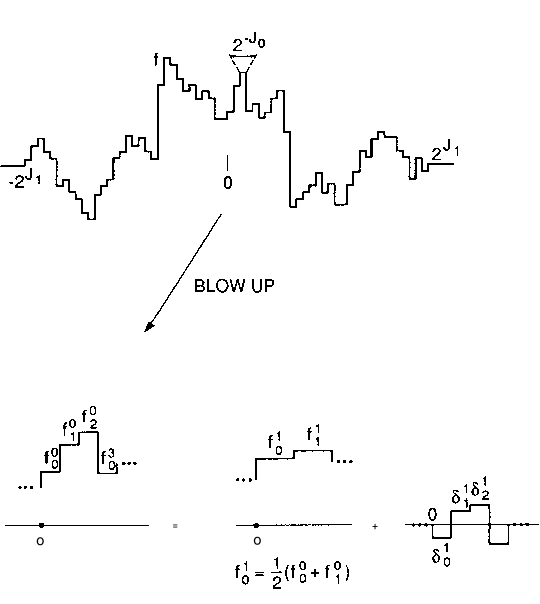
\includegraphics{HaarWavelet.png}}
  \caption{\label{fig:blowup}(upper) A function $f$ with support $[- 2^{J_1},
  2^{J_1}]$, piecewise constant on the $[\ell 2^{- J_0}, (\ell + 1) 2^{- J_0})
  .$ (lower) A blowup of a portion of $f$.}
\end{figure}

We can apply the same trick to $f^1$, so that
\[ f^1 = f^2 + \sum_l c_{- J_0 + 2, \ell} \psi_{- J_0 + 2, \ell} . \]
We keep going the trick until we have
\[ f = f^{J_0 + J_1} + \sum_{m = - J_0 + 1}^{J_1} \sum_{\ell} c_{m, \ell}
   \psi_{m, \ell} . \]
Here $f^{J_0 + J_1}$ consists of two constant pieces (see Figure
\ref{fig:haarWavelet2}).

\begin{figure}[h]
  \resizebox{278px}{202px}{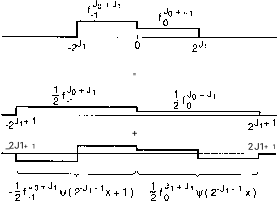
\includegraphics{HaarWavelet2.png}}
  \caption{\label{fig:haarWavelet2}Extending interval $[- 2^{J_1}, 2^{J_1}]$
  to $[- 2^{J_1 + 1}, 2^{J_1 + 1}]$.}
\end{figure}

As is shown in Figure \ref{fig:haarWavelet2}, the interval can be extended to
twice larger, which means the support of function $f$ is extended:
\[ f = f^{J_0 + J_1 + K} + \sum_{m = - J_0 + 1}^{J_1 + K} \sum_{\ell} c_{m,
   \ell} \psi_{m, \ell} . \]
It follows immediately that
\begin{eqnarray*}
  \left\| f - \sum_{m = - J_0 + 1}^{J_1 + K} \sum_{\ell} c_{m, \ell} \psi_{m,
  \ell} \right\|_{L^2}^2 & = & \| f^{J_0 + J_1 + K} \|_{L^2}^2\\
  & = & 2^{- K / 2} \cdot 2^{J_1 / 2} (| f_0^{J_0 + J_1} |^2 + | f_{- 1}^{J_0
  + J_1} |^2)^{1 / 2},
\end{eqnarray*}
which can be arbitrarily small by taking sufficiently large $K$. Finally, this
illustrates that $f$ can be approximated to arbitrary precision by a finite
linear combination of Haar wavelets.

\subsection{Scaling Function}

The core part of wavelet analysis is the wavelet transform which is a tool
that split data, function or operator into components with different
frequency, and then studies the above componet with a resolution matched to
its scale{\cite{williams1994introduction,daubechies1992ten}}. The spliting of
data, function or operator is described mathematically with multiresolution of
a functional space defined below.

In order to develop a multilevel representation of a function in $L^2
(\mathbbm{R})$, we seek a squence of embedded subspaces $V_i$ such that
\begin{equation}
  \{ 0 \} \subset \cdots \subset V_{- 1} \subset V_0 \subset V_1 \subset V_2
  \subset \cdots \subset L^2 (\mathbbm{R})
\end{equation}
with the following properties:
\begin{itemize}
  \item $\bigcup_{j \in \mathbbm{Z}} V_j$ is dense in $L^2 (\mathbbm{R}) .$
  
  \item $\bigcap_{j \in \mathbbm{Z}} V_j = \{ 0 \} .$
  
  \item The embedded subspaces are related by a scaling law
  \[ g (x) \in V_j \quad \Leftrightarrow \quad g (2 x) \in V_{j + 1} \]
  \item Each subspace is spanned by integer translates of a single function $g
  (x)$ such that
  \[ g (x) \in V_0 \quad \Leftrightarrow \quad g (x + 1) \in V_0 \]
\end{itemize}
\begin{definition}[Multiresolution Analysis]
  If there exists function $\phi (x) \in V_0 $ such that its integer
  translates $\{ \phi (x - k) \}_{k \in \mathbbm{Z}}$ form a Riesz
  basis\footnote{Sequence $\{ x_k \}_{k \in \mathbbm{Z}}$ forms a Riesz
  squence of a Hilbert space $\mathcal{H}$ if there exists constants $0 < c <
  C < + \infty$ such that
  \[ c \left( \sum_n | a_n |^2 \right) \leqslant \left\| \sum_n a_n x_n
     \right\|^2 \leqslant C \left( \sum_n | a_n |^2 \right) \]
  for all sequences $\{ a_k \}_{k \in \mathbbm{Z}} \subset l^2$, and a Riesz
  squence $\{ x_k \}_{k \in \mathbbm{Z}}$ forms a Riesz basis if
  \[ \overline{\tmop{span} (x_k)} =\mathcal{H}. \]
  \[ \  \]} for the space $V_0$, then the sequence of subspaces $\{ V_j \}_{j
  \in \mathbbm{Z}}$ forms a multiresolution analysis of $L^2 (\mathbbm{R})$
  space.
\end{definition}

\begin{definition}[Scaling Function]
  The function $\phi (x)$ is called scaling function if it produces a
  multiresolution of $L^2 (\mathbbm{R}) .$
\end{definition}

It can be proved that $\{ \nobracket \phi (2 x - k \}_{k \in \mathbbm{Z}}$
form a basis for the space $V_1$\footnote{Scaling by power other than 2 is
also feasible.}. Thus,
\begin{eqnarray*}
  V_0 = & \overline{\tmop{span} \{ \phi (x - k) \}_{k \in \mathbbm{Z}}} & \\
  V_1 = & \overline{\tmop{span} \{ \phi (2 x - k) \}_{k \in \mathbbm{Z}}} & .
\end{eqnarray*}
Since $V_0 \subset V_1$, we have the following \tmtextit{dilation equation}:
\begin{equation}
  \phi (x) = \sum_{k = - \infty}^{+ \infty} a_k \phi (2 x - k), \quad \{ a_k
  \}_{k \in \mathbbm{Z}} \subset l^2 (\mathbbm{R}) . \label{dilation}
\end{equation}
Similarly we can define
\begin{equation}
  \phi_{m, k} (x) = 2^{m / 2} \phi (2^m x - k)
\end{equation}
then it can be deduced that $\{ \phi_{m, k} (x) \}_{k \in \mathbbm{Z}}$ form a
Riesz basis for the space $V_m$.

If the integer translates of scaling function $\{ \phi (x - k) \}_{k \in
\mathbbm{Z}}$ is further constrained as being orthonormal basis of space
$V_0$, then we have $\{ \phi_{m, k} (x) \}_{k \in \mathbbm{Z}}$ forming an
orthonormal basis of space $V_m$. The dilation parameter $m$ is referred to as
the \tmtextit{scale}.

\subsection{Wavelet}

The concept \tmtextit{wavelet} comes from the difference between subspace
$V_{m - 1}$ and $V_m$. The subspace $W_{m - 1}$ of $L^2 (\mathbbm{R})$ is
defined as the orthogonal complement of $V_{m - 1}$ in $V_m$:
\begin{equation}
  V_m = V_{m - 1} \oplus W_{m - 1} .
\end{equation}
It follows that the spaces $W_j$ are orthogonal and that
\begin{equation}
  \bigoplus_{j \in \mathbbm{Z}} W_j = L^2 (\mathbbm{R}) .
\end{equation}
\begin{definition}[Wavelet]
  Similar to the definition of scaling function to subspace $V_0$, a wavelet
  function $\psi (x)$ can be introduced such that $\{ \psi (x - k) \}_{k \in
  \mathbbm{Z}}$ forms a Riesz basis for subspace $W_0$.Then
  \begin{equation}
    \psi_{m, k} (x) = 2^{m / 2} \psi (2^m x - k) \quad m, k \in \mathbbm{Z}
  \end{equation}
  forming a Riesz basis for subspace $W_m$ is defined as a wavelet in $L^2
  (\mathbbm{R})$.
\end{definition}

After defining the multiresolution analysis and wavelet, two projection
operators can be introduced, assuming that $\{ \phi_{m, k} (x) \}_{k \in
\mathbbm{Z}}$ and $\{ \psi_{m, k} (x) \}_{k \in \mathbbm{Z}}$ are both
orthonormal basis. We may now approximate a function $f \in L^2 (\mathbbm{R})$
by its projection
\begin{equation}
  P_m f (x) = \sum_{k = - \infty}^{+ \infty} c_{m, k} \phi_{m, k} (x),
  \label{expansion-pm}
\end{equation}
we may also define projection of function $f$ on subspace $W_m$ as $Q_m$ and
it follows that
\begin{equation}
  P_m = P_{m - 1} + Q_{m - 1} . \label{pq-relationship}
\end{equation}
This implies that $Q_m f$ is represents the details that was lost from one
level of approximation to a coarser level.

The multiresolution analysis defined in a functional way can be explained as
follows. If we have the expansion coefficients $c_{m, k}$ in equation
(\ref{expansion-pm}), then we can decomposes them into two parts with equation
(\ref{pq-relationship}):
\begin{enumeratenumeric}
  \item the expansion coefficients $c_{m - 1, k}$ of the approximation $P_{m -
  1} f$,
  
  \item the expansion coefficients $d_{m - 1, k}$ of the detail component
  $Q_{m - 1} f.$
\end{enumeratenumeric}

\chapter{Construction and Properties of Wavelet System}

This chapter is mainly according to {\cite{williams1994introduction}}.

\section{The Construction of Daubechies Wavelet System}

\subsection{Quadrature Mirror Filters}

In general, a scaling function $\phi (x)$ is solution to dilation equation
(\ref{dilation}), and the constants $a_k$ are called filter coefficients and
it is often the case that only a finite number of these are non-zero. Given
the filter coefficients, the scaling function can be deduced, and the
corresponding wavelet transform is determined; if certain conditions are
imposed on the scaling functions, the filter coefficients can be fully
derived, and this is the most important contribution of modern wavelet theory
(along with frame theory).

One of the most important condition on scaling function is orthogonality:
\[ \int_{- \infty}^{\infty} \phi (x) \phi (x + l) \mathd x = \delta_{0, l}
   \quad l \in \mathbbm{Z}, \]
so a wavelet being orthogonal to the scaling function can defined by:
\[ \psi (x) = \sum_{k = - \infty}^{+ \infty} (- 1)^k a_{N - 1 - k} \phi (2 x -
   k) \]
where $N$ is an even integer\footnote{It will then be shown that the wavelet
has support over $[0, N - 1]$.}. The orthogonality is verified as follows:
\begin{eqnarray*}
  \langle \phi (x), \psi (x) \rangle & = & \int_{- \infty}^{\infty} \sum_{k =
  - \infty}^{+ \infty} a_k \phi (2 x - k) \sum_{l = - \infty}^{+ \infty} (-
  1)^l a_{N - 1 - l} \phi (2 x - l)\\
  & = & \frac{1}{2} \sum_{k = - \infty}^{+ \infty} (- 1)^k a_{N - 1 - k}
  a_k\\
  & = & 0.
\end{eqnarray*}
The set of coefficients $\{ a_k \}$ and $\{ (- 1)^k a_{N - 1 - k} \}$ are said
to form a pair of \tmtextit{quadrature mirror filters}.

\subsection{Derivation of Filter Coefficients}

There are several properties that are essential to a useful basis for
functional analysis which lead to the corresponding conditions constraining
the filter coefficients. They are listed below:
\begin{enumeratenumeric}
  \item Normalization to unity, i.e.
  \[ \int_{- \infty}^{+ \infty} \phi (x) \mathd x = 1, \]
  which leads to
  \begin{equation}
    \sum_{k = - \infty}^{+ \infty} a_k = 2. \label{normal-cond}
  \end{equation}
  \item Orthogonality of scaling function, i.e.
  \[ \int_{- \infty}^{+ \infty} \phi (x) \phi (x + l) \mathd x = \delta_{0, l}
     \quad l \in \mathbbm{Z}, \]
  which yields
  \begin{equation}
    \sum_{k = - \infty}^{+ \infty} a_k a_{k + 2 l} = 2 \delta_{0, l} \quad l
    \in \mathbbm{Z}. \label{orthogonal-cond}
  \end{equation}
  \item Vanishing moment, i.e.
  \[ \int_{- \infty}^{+ \infty} \psi (x) x^l \mathd x = 0 \quad l = 0, 1, 2,
     \ldots, p - 1, \]
  which yields (by Daubechies {\cite{daubechies1992ten}})
  \begin{equation}
    \sum_{k = - \infty}^{+ \infty} (- 1)^k a_k k^l = 0 \quad l = 0, 1, 2,
    \ldots, N / 2 - 1 \label{vanishing-cond},
  \end{equation}
  and a more detailed discussion on equation (\ref{vanishing-cond}) can be
  found in {\cite{williams1994introduction}}.
\end{enumeratenumeric}
The filter coefficients $\{ a_k \}_{k = 0, 1, \ldots, N - 1}$ for an N
coefficient system are uniquely defined by equation (\ref{normal-cond},
\ref{orthogonal-cond}, and \ref{vanishing-cond}).

\subsection{Construction of Scaling Function}

In general, there is no closed-form solution of scaling function, and they
have to be attained recursively from the dilation equation (\ref{dilation})
instead. In the case of quadrature mirror filter:
\[ \phi (x) = a_{_0} \phi (2 x) + a_1 \phi (2 x - 1) + a_2 \phi (2 x - 2) +
   \cdots + a_{N - 1} \phi (2 x - N + 1), \]
and it can be proved that{\cite{williams1994introduction}} all integer points
outside $[0, N - 1]$ have zero value, we have
\begin{eqnarray*}
  \phi (0) & = & a_0 \phi (0)\\
  \phi (1) & = & a_0 \phi (2) + a_1 \phi (1) + a_2 \phi (0)\\
  \phi (2) & = & a_0 \phi (4) + a_1 \phi (3) + a_2 \phi (2) + a_3 \phi (1) +
  a_4 \phi (0)\\
  & \vdots & \\
  \phi (N - 2) & = & a_{N - 3} \phi (N - 1) + a_{N - 2} \phi (N - 2) + a_{N -
  1} \phi (N - 3)\\
  \phi (N - 1) & = & a_{N - 1} \phi (N - 1) .
\end{eqnarray*}
or
\[ M \Phi = \Phi \]
This linear equation system is actually finding the eigenvector of matrix $M$
corresponding to the eigenvalue $1$, so the normalizing condition is
necessary:
\[ \sum_{k = - \infty}^{+ \infty} \phi (i) = 1 \quad i \in \mathbbm{Z}. \]


The above process gives the scaling function on integer points, and the
scaling function on all real points can be calculated by bisection method:
\[ \phi \left( \frac{x}{2} \right) = \sum_{k = - \infty}^{+ \infty} a_k \phi
   (x - k) . \]

\subsection{Example: The Daubechies 4 Coefficient Wavelet System}

Here we demonstrate the construction of the so called D4 Wavelet. According to
equation (\ref{normal-cond}, \ref{orthogonal-cond}, \ref{vanishing-cond}), we
have
\begin{eqnarray*}
  a_0 + a_1 + a_2 + a_3 & = & 2\\
  a_0^2 + a_1^2 + a_2^2 + a_3^2 & = & 2\\
  a_0 - a_1 + a_2 - a_3 & = & 0\\
  - a_1 + 2 a_2 - 3 a_3 & = & 0
\end{eqnarray*}
One set of solution is \begin{eqnarray*}
  a_0 & = & \frac{1 + \sqrt{3}}{4}\\
  a_1 & = & \frac{3 + \sqrt{3}}{4}\\
  a_2 & = & \frac{3 - \sqrt{3}}{4}\\
  a_3 & = & \frac{1 - \sqrt{3}}{4}
\end{eqnarray*}

and the other set of solution is the antithesis of this set leading to $\phi
(- x)$ instead of $\phi (x)$.

The values of the scaling function on integer points are given by
\[ \left[\begin{array}{cccc}
     a_0 - 1 & 0 & 0 & 0\\
     a_2 & a_1 - 1 & a_0 & 0\\
     0 & a_3 & a_2 - 1 & a_1\\
     0 & 0 & 0 & a_3 - 1
   \end{array}\right] \left[\begin{array}{c}
     \phi (0)\\
     \phi (1)\\
     \phi (2)\\
     \phi (3)
   \end{array}\right] = \left[\begin{array}{c}
     0\\
     0\\
     0\\
     0
   \end{array}\right] \]
and solved as:
\[ \phi (0) = 0 \quad \phi (1) = \frac{1 + \sqrt{3}}{2} \quad \phi (2) =
   \frac{1 - \sqrt{3}}{2} \quad \phi (3) = 0. \]
Additionally we have the half integers:
\begin{eqnarray*}
  \phi \left( \frac{1}{2} \right) & = & a_0 \phi (1) = \frac{2 +
  \sqrt{3}}{4}\\
  \phi \left( \frac{3}{2} \right) & = & a_1 \phi (2) + a_2 \phi (1) = 0\\
  \phi \left( \frac{5}{2} \right) & = & a_3 \phi (2) = \frac{2 - \sqrt{3}}{4}
  .
\end{eqnarray*}
Any real number point on $[0, 3]$ can be calculated similarly, and it can be
verified easily that the scaling function always has null value outside $[0,
3]$, which means it has compact support.

\section{Classification of Wavelet Bases}

There are many families of orthogonal wavelets that have been constructed in
$L^2 (\mathbbm{R})$. We can classify them with the following criteria:
localization in physical space (owing to their fast decay or even compact
support{\cite{schneider2010wavelet}}), localization in frequency space (owing
to their vanishing moments and smoothness{\cite{schneider2010wavelet}}),
continuity, and differentiablity.

\section{Mallat Transform}

The Mallat Transform provides a simple means of transforming data from one
level of resolution $m$ to the next coarser level of resolution $m - 1$. The
inverse Mallat transform is a transform from the coarser level $m - 1$ back to
the finer level $m$.

\subsection{Multiresolution Decomposition}

As is mentioned before, the multiresolution decomposition consists of two
parts:
\begin{enumeratenumeric}
  \item the expansion coefficients $c_{m - 1, k}$ of the approximation $P_{m -
  1} f$,
  
  \item the expansion coefficients $d_{m - 1, k}$ of the detail component
  $Q_{m - 1} f.$
\end{enumeratenumeric}
Consider a function $f$:
\begin{eqnarray*}
  P_m f & = & \sum_{k = - \infty}^{+ \infty} c_{m, k} \phi_{m, k} (x) \quad
  c_{m, k} = \langle f, \nospace \phi_{m, k} \rangle\\
  Q_m f & = & \sum_{k = - \infty}^{+ \infty} d_{m, k} \psi_{m, k} (x) \quad
  d_{m, k} = \langle f, \psi_{m, k} \rangle\\
  P_{m - 1} f & = & P_m f - Q_{m - 1} f.
\end{eqnarray*}
Substituting the above in
\[ c_{m - 1, k} = \langle P_{m - 1} f, \phi_{m - 1, k} \rangle \]
leads to the following result
\begin{equation}
  c_{m - 1, k} = \frac{1}{\sqrt{2}} \sum_{j = - \infty}^{+ \infty} c_{m, j}
  a_{j - 2 k} \label{MallatTransC} .
\end{equation}
\[ \  \]
Similarly there is:
\begin{equation}
  d_{m - 1, k} = \frac{1}{\sqrt{2}} \sum_{j = - \infty}^{+ \infty} c_{m, j} (-
  1)^{^j} a_{N - 1 - j + 2 k} \label{MallatTransD} .
\end{equation}
Equation (\ref{MallatTransC}, \ref{MallatTransD}) form the basis of the Mallat
transform algorithm.

\subsection{Multiresolution Reconstruction}

Multiresolution construction use $c_{m - 1, k}$ and $d_{m - 1, k}$ to
reconstruct $c_{m, k}$. Considering the following relationship:
\begin{eqnarray*}
  P_m f & = & P_{m - 1} f + Q_{m - 1} f\\
  c_{m, k} & = & \langle P_m f, \phi_{m, k} \rangle
\end{eqnarray*}
leads to
\begin{equation}
  c_{m, k} = \frac{1}{\sqrt{2}} \sum_{j = - \infty}^{+ \infty} c_{m - 1, j}
  a_{k - 2 j} + \frac{1}{\sqrt{2}} \sum_{j = - \infty}^{+ \infty} d_{m - 1, k}
  (- 1)^k a_{N - 1 - k + 2 j} \label{InverseMallatTrans} .
\end{equation}
Equation (\ref{InverseMallatTrans}) forms the basis of the inverse Mallat
transform algorithm.

\subsection{The Mallat Transform and Inverse Transform Algorithm}

The equations (\ref{MallatTransC}, \ref{MallatTransD}, and
\ref{InverseMallatTrans}) is expressed by the following algorithm. Consider a
string of data $c_{m, k}$ of finite length $n$ which represents the
approximation $P_m f$ to a function. For convenience, suppose that this data
is periodic with period $n$. The matrix form of equation (\ref{MallatTransC})
is
\[ \left[\begin{array}{c}
     c_{m - 1, 0}\\
     \times\\
     c_{m - 1, 1}\\
     \times\\
     c_{m - 1, 2}\\
     \times\\
     \cdots\\
     \cdots\\
     c_{m - 1, n / 2 - 1}\\
     \times
   \end{array}\right] = \frac{1}{\sqrt{2}} \left[\begin{array}{cccccccc}
     a_0 & a_1 & a_2 & a_3 & \cdots & a_{N - 1} & \cdots & 0\\
     0 & a_0 & a_1 & a_2 & \cdots & a_{N - 2} & \cdots & 0\\
     0 & 0 & a_0 & a_1 & \cdots & a_{N - 3} & \cdots & 0\\
     0 & 0 & 0 & a_0 & \cdots & a_{N - 4} & \cdots & 0\\
     \cdots & \cdots & \cdots & \cdots & \cdots & \cdots & \cdots & \cdots\\
     0 & 0 & 0 & 0 & \cdots & \cdots & \cdots & a_{N - 1}\\
     a_{N - 1} & 0 & 0 & 0 & \cdots & \cdots & \cdots & a_{N - 2}\\
     \cdots & \cdots & \cdots & \cdots & \cdots & \cdots & \cdots & \cdots\\
     a_2 & a_3 & a_4 & a_5 & \cdots & 0 & \cdots & a_1\\
     a_1 & a_2 & a_3 & a_4 & \cdots & 0 & \cdots & a_0
   \end{array}\right] \left[\begin{array}{c}
     c_{m, 0}\\
     c_{m, 1}\\
     c_{m, 2}\\
     c_{m, 3}\\
     \cdots\\
     \cdots\\
     \cdots\\
     \cdots\\
     c_{m, n - 2}\\
     c_{m, n - 1}
   \end{array}\right] \]
in which $\times$ represents information of no value. The matrix of filter
coefficients is a circulant matrix, so that the right-hand side of the
equation is effectively a convolution of the discrete filter
\[ \tilde{h} = \frac{1}{\sqrt{2}} [a_0, 0, 0, 0, \ldots, 0, a_{N - 1}, \ldots,
   a_2, a_1]^{\Tau} \]
with the data $c_{m, k}$. Only every other sample of the result needs be kept;
this process is called decimation. Similarly, the $d_{m - 1, k}$ is
effectively a convolution of the discrete filter
\[ \tilde{g} = \frac{1}{\sqrt{2}} [a_{N - 1}, 0, 0, 0, \ldots, 0, - a_0,
   \ldots, a_{N - 3}, - a_{N - 2}]^{\Tau} \]
with the data $c_{m, k}$. The above two steps constitutes the Mallat transform
(decomposition). The reconstruction algorithm can allso be obtained by the
matrix form of equation (\ref{InverseMallatTrans}):
\begin{enumerate}
  \item insert a zero between every sample in $c_{m - 1, k}$ and $d_{m - 1,
  k}$,
  
  \item convolve $c_{m - 1, k}$ with the filter $h$,
  
  \item convolve $d_{m - 1, k}$ with the filter $g$,
  
  \item add results in 2. and 3. to get the original data, $c_{m, k}$,
\end{enumerate}
where the filters $h$ and $g$ are
\[ h = \frac{1}{\sqrt{2}} [a_0, a_1, a_2, a_3, \ldots, a_{N - 2}, a_{N - 1},
   \ldots, 0, 0]^{\Tau} \]
and
\[ g = \frac{1}{\sqrt{2}} [a_{N - 1}, - a_{N - 2}, a_{N - 3}, - a_{N - 4},
   \ldots, a_1, - a_0, \ldots, 0, 0]^{\Tau} \]

\chapter{Wavelet in Numerical Analysis}

\section{Some Useful Orthogonal Wavelets}

\part{Application of Wavelet Analysis in CFD}

\chapter{Miscellaneous Staff}

\section{Orthogonal Wavelet with Gaussian Distribution as Scaling Function?}

The answer is that this is not feasible. Suppose we have
\[ \phi (x) = \frac{1}{\sqrt{2 \mathpi}} \mathe^{- \frac{(x - x_0)^2}{2}}, \]
then it can be calculated that
\[ \hat{\phi} (\gamma) = \int_{- \infty}^{+ \infty} \phi (x) \mathe^{- 2
   \mathpi \mathi \gamma x} \mathd x = \mathe^{- 2 \mathpi \gamma (\mathi x_0
   + 2 \mathpi \gamma)} . \]
However we have also
\[ H_0 (\gamma) = \frac{\hat{\phi} (2 \gamma)}{\hat{\phi} (\gamma)} =
   \mathe^{- 6 \mathpi^2 \gamma^2} \mathe^{- 2 \mathpi \mathi \gamma x_0} \]
which is not 1-periodic: this violates theorem \ref{thm:constructionMRA}. So
it is important to construct an orthogonal wavelet with Gaussian distriubtion
as its scaling function.

\begin{thebibliography}{1}
  \bibitem[1]{WangJizeng2001}王记增.{\newblock}
  \tmtextit{正交小波统一理论与方法及其在压电智能结构等力学研究中的应用
  [D]}.{\newblock} PhD thesis , 2001.{\newblock}
  
  \bibitem[2]{christensen2010functions}Ole Christensen.{\newblock}
  \tmtextit{Functions, spaces, and expansions: mathematical tools in physics
  and engineering}.{\newblock} Springer Science \& Business Media,
  2010.{\newblock}
  
  \bibitem[3]{daubechies1992ten}Ingrid Daubechies.{\newblock} \tmtextit{Ten
  lectures on wavelets}.{\newblock} SIAM, 1992.{\newblock}
  
  \bibitem[4]{schneider2010wavelet}Kai Schneider  and  Oleg~V
  Vasilyev.{\newblock} Wavelet methods in computational fluid
  dynamics.{\newblock} \tmtextit{Annual Review of Fluid Mechanics},
  42:473--503, 2010.{\newblock}
  
  \bibitem[5]{williams1994introduction}John~R Williams  and  Kevin
  Amaratunga.{\newblock} Introduction to wavelets in engineering.{\newblock}
  \tmtextit{International journal for numerical methods in engineering},
  37(14):2365--2388, 1994.{\newblock}
  
  \bibitem[6]{walnut2013introduction}David~F Walnut.{\newblock} \tmtextit{An
  introduction to wavelet analysis}.{\newblock} Springer Science \& Business
  Media, 2013.{\newblock}
\end{thebibliography}

\end{document}
